\chapter{Methods}
To initiate the process of identifying the most promising models for time series classification, a comprehensive review of the current state of the art in the field was conducted.
This involved a meticulous exploration of published research studies and academic papers related to the research question.
Subsequently, the different approaches presented in the literature were thoroughly analyzed and compared, following the most promising models were shortlisted for further examination and testing.

Once the model selection phase was completed, I proceeded to conduct an in-depth study of the papers and any available source code.
This was done to enhance their understanding of the underlying algorithms and techniques employed in each model, as well as any implementation details that may be relevant for adapting to the specific research needs.

As a result of these efforts, four models - Random Forest (RF), Adversarial Joint-Learning Recurrent Neural Network (AJ-RNN), Temporal Convolutional Neural Network (TempCNN), and Lightweight Temporal Self-Attention Encoder (L-TAE) - were evaluated in this study, and their details are presented in this section.


\section{Random forest}

TensorFlow Decision Forests (TF-DF) \cite{TensorFlow:rf} is the library used to train and evaluate the random forest model.

A Random Forest \cite{breiman2001random} is a collection of deep CART decision trees trained independently and without pruning.
Each tree is trained on a random subset of the original training dataset (sampled with replacement).
The algorithm is unique in that it is robust to overfitting, even in extreme cases e.g. when there are more features than training examples.
It is probably the most well-known of the Decision Forest training algorithms.

\pagebreak
\section{TempCNN}

The article ``Temporal Convolutional Neural Network for the Classification of Satellite Image Time Series'' \cite{tempCNN} presents a machine learning model for classifying satellite image time series data.
The model is based on Convolutional Neural Networks (CNNs) and aims to improve traditional image classification methods by incorporating time series information into the model.

The Temporal Convolutional Neural Network (TempCNN) architecture was used in the following experiments to classify satellite image time series.

The model inputs a series of satellite images and applies a series of convolutional and pooling operations to extract high-level features from the data.
The paper presents a novel approach to classify satellite image time series data and highlights the potential applications of the model in areas such as remote sensing and environmental monitoring.

\subsection{Temporal Convolutions}
% TODO: review
Convolutional layers have been proposed as a technique to limit the number of weights a network must learn while exploiting structural dimensions in the data, such as spatial, temporal, or spectral dimensions \cite{NIPS1989_53c3bce6}. 
These layers apply a convolution filter to the output of the previous layer, resulting in an activation map as output, rather than a single activation value per neuron as in dense (fully connected) layers.
For example, with a univariate time series as input, the output of the convolutional layer would be a new time series, with each data point generated by the corresponding convolution filter applied to the original series.

Convolutional layers have the property of sharing their parameters across locations.
This characteristic involves applying the same linear combination by sliding it over the input, resulting in a significant reduction in the number of weights in the layer. 
This reduction is based on the assumption that the same convolution can be beneficial in different parts of the time series.
Therefore, the number of trainable parameters depends only on the filter size of the convolution and the number of units, but not on the input size.

The output size, on the other hand, depends on the input size, the stride, and the padding.
The stride controls the interval between two convolution centers, while padding controls the addition of values (usually zeros) at the beginning and end of the input series before computing the convolution. 
Padding can guarantee that the output is the same size as the input.


\subsection{Model}

The baseline architecture of TempCNN used for the experiments, as shown in Figure \ref{fig:temCNNArchitecture}, consists of three convolutional layers (64 units), one dense layer (256 units), and one softmax layer.
In the experimental section, we will investigate the width (i.e., number of units) of the convolutional layers, the depth (i.e., number of convolutional layers), and the pooling layers of the network.

\begin{figure}[H]
  \centering
  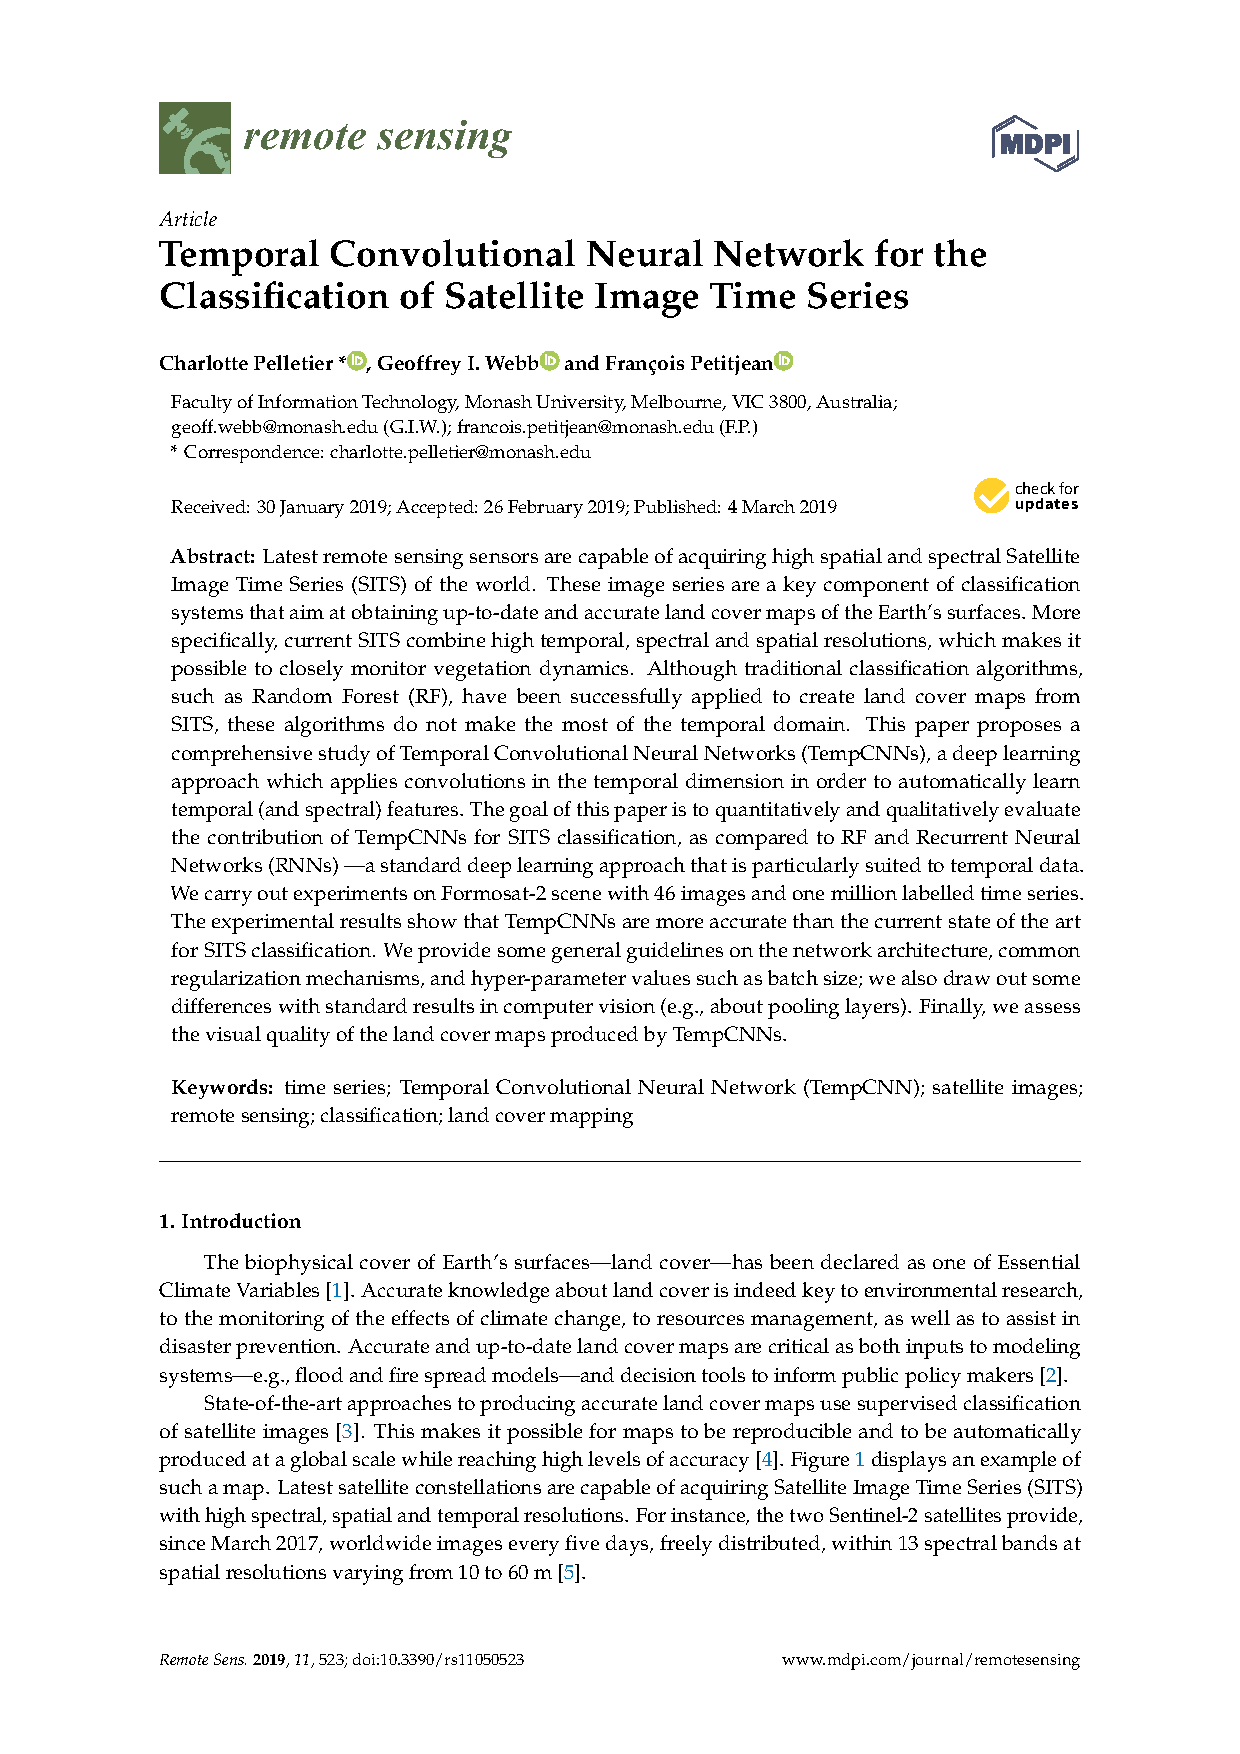
\includegraphics[width=1\textwidth]{tempCNN}
  \caption{Proposed temporal Convolutional Neural Network (TempCNN). The network input is a
  multi-variate time series. Three convolutional filters are consecutively applied, then one dense layer,
  and finally the Softmax layer, that provides the predicting class distribution.    \cite{tempCNN}}
  \label{fig:temCNNArchitecture}
\end{figure}


To prevent overfitting, we employed the same regularization mechanisms described in \cite{tempCNN}:

\begin{itemize}
  \item dropout rate of 0.5 \cite{JMLR:v15:srivastava14a}. 
  \item L2-regularization on the weights (also named weight-decay) applied for all the layers with a small rate of $10^{-6}$ 
  \item batch normalization \cite{DBLP:journals/corr/IoffeS15}.
\end{itemize}

To train the network Adam optimization was used with the standard parameter values: $\beta_1 = 0.9$, $\beta_2 = 0.999$, and $e = 10^{-8}$) \cite{kingma2014adam} 
We used a batch size of 32, and a maximum number of epochs set to 20, with an early stopping mechanism with a patience of zero on the validation loss. 



\pagebreak
\section{AJ-RNN}
``Adversarial Joint-Learning Recurrent Neural Network for Incomplete Time Series Classification" \cite{ajrnn} is a research paper that proposes a novel approach for classification of incomplete time series data.
The authors begin by highlighting the challenges of working with incomplete time series data, particularly the difficulty of extracting features and the need to deal with missing values.

To address these challenges, the authors propose an adversarial joint-learning recurrent neural network (AJ-RNN) that uses a recurrent neural network (RNN) to capture the temporal dependencies in the time series data, and an adversarial learning approach to impute the missing values.

The AJ-RNN is trained using a joint optimization framework that alternates between training the RNN for classification and the imputation network to fill in the missing values.
The adversarial component of the imputation network is used to ensure that the imputed values are as close as possible to the true values.

The authors evaluate the performance of the AJ-RNN on several real-world datasets and demonstrate that it outperforms several existing state-of-the-art approaches for time series classification.

\subsection{Adversarial learning}

Previous studies have shown that adversarial approaches outperform traditional methods in generating data that conforms to the distribution of a given dataset \cite{goodfellow2014generative, ledig2017photo}.

Furthermore, GANs have shown promising results in filling in missing data in time series prediction \cite{yoon2018gain, li2018learning, luo2018multivariate}. Similarly, adversarial techniques have also been applied to tasks such as video captioning \cite{yang2018video} and domain adaptation \cite{ganin2017domain}.
However, prior to this paper, the question of how to apply adversarial learning in the domain of incomplete time series classification (ITSC) has not been explored.

The integration of adversarial training and joint learning in recurrent neural networks (RNNs) is explored in this paper, resulting in the development of a system called Adversarial Joint learning RNN (AJ-RNN).

The study's results show that employing AJ-RNN, an end-to-end framework integrating adversarial training and joint learning in recurrent neural networks, is an effective solution to tackle the issue of incomplete time series classification.
AJ-RNN is trained to predict the value of the next input variable when it is revealed, and to fill in the missing value with its prediction.
At the same time, AJ-RNN also learns to classify.
Hence AJ-RNN can directly perform classification with missing values.

\subsection{Model}


The following section presents the Adversarial Joint learning Recurrent Neural Network (AJ-RNN) as a solution for time series classification with missing values. 
The architecture of the model is illustrated in Figure \ref{fig:AJRNNrchitecture}. 

Here we describe how adversarial and joint learning strategies are integrated into an RNN.


The time series $X$ is represented as a sequence vector of $T$ observations, denoted by $X = \{x_1, x_2, ..., x_T \}$. Each observation $x_t \in R^d$ is a $d$-dimensional vector.

Assume that a time series $X$ has missing values which are represented by a $T$-dimensional mask vector $M = \{m_1, m_2, ..., m_T\}$.
The elements $m_t$ of the mask vector are binary values indicating the presence or absence of the corresponding element $x_t$ in the time series, where $m_t$ takes the value of $1$ if $x_t$ is revealed and $0$ if $x_t$ is missing.

Each time series $X^i$ in the dataset $D$ is associated with a target label $y^{(i)}$, and a mask vector $M^i$, where $D = {(X^i,M^i, y^i)}^N_{i=1}$.

To avoid the traditional two-step approach, imputation and classification are regarded as two tasks in multitask learning.

The AJ-RNN is trained to approximate the value of the next input variable and use it as a target when it is revealed.
If the next value is missing, it is filled in with the current prediction.
At the same time, the AJ-RNN is trained to perform the classification task.

The missing value problem is addressed through two processes, namely approximation and imputation.
As shown in Figure \ref{fig:AJRNNrchitecture}, two kinds of links enable AJ-RNN to directly model time series in the presence of missing values: dashed blue links (for approximation) and solid blue links (for imputation). 
The system is trained to approximate the next value $x_t$ using the last hidden state $h_{t-1}$ as follows:

\begin{equation}
  \hat{x_t} = W_{imp} h_{t-1} + b_z
\end{equation}

where $W_{imp} \in R^{n \times  m}$ is a learned regression matrix and $b_z$ is a bias term. 
As $\hat{x_t}$ is trained to approximate the next value $x_t$, it can be employed for imputing it when it is missing.
The input value $u_t$ is computed as:

\begin{equation}
  u_t = m_t \odot x_t + (1 - m_t) \odot \hat{x_t}
  \label{eq:AJRNNinput}
\end{equation}

where $m_t$ is the mask as defined above and $\odot$ is the element-wise product.

The completed input value $u_t$ is used to train the RNN.
The update equation of the RNN is:

\begin{equation}
  h_t = F_{RNN} (h_{t-1}, u_t; W)
\end{equation}

Where $h_t$ represents the hidden unit vector at time $t$, $W$ encapsulates the input-to-hidden and hidden-to-hidden parameters, and $F_{RNN}$ represents the update function of the particular RNN variant.

To obtain the probability distribution over each category label, a softmax is applied to the output of the classifier, which takes the last hidden state of the RNN, $h_T$, as input.

\begin{equation}
  P(\hat{y_j}|h_T ) = \frac{exp(W^T_j  h_T )}{\sum_{l=1}^K exp(W^T_l  h_T )}
  \label{eq:AJRNNsoftmax}
\end{equation}

where $K$ is the number of class labels and $\{W_l\}^K_{l=1}$ are the class-specific weights of the softmax layer.
More complex networks can be used for the classifier based on the specific task at hand. However, in this study, a simple classifier is used.

During joint learning, imputation and classification tasks are performed. 
Let $D$ be the time series dataset and let the superscript $i$ denote the $i$-th sample in the dataset.
The imputation task produces an imputation sequence vector $\hat{X^i} = { \hat{x}^i_2, ..., \hat{x}^i_T }$ for the $i$-th time series sample.
This vector is composed of two parts: approximation values (represented by orange units in Fig. \ref{fig:AJRNNrchitecture}) and imputation values (represented by purple units in Fig. \ref{fig:AJRNNrchitecture}).  
The imputation loss of all time series samples is calculated on the approximation values as follows:

\begin{equation}
  \mathcal{L}_{imp}(X, \hat{X}, M) = \frac{1}{N} \sum_{i=1}^N \lVert (X^i_{2:T} - \hat{X}^i) \odot M^i_{2:T} \rVert_2^2
  \label{eq:AJRNNimploss}
\end{equation}

where $N$ represents the number of samples in the dataset.
Equation (\ref{eq:AJRNNimploss}) measures the mean squared error loss between the approximation and the revealed values.
The mask $M^i_{2:T}$ is used to ignore the imputation values in the loss calculation, as there is no ground truth available for these missing values.


The loss for the classification task can be calculated as follows. 
Let $y^i$ be the true label of the $i$-th time series sample and $\hat{y}^i$ be the predicted probability distribution given by Equation (\ref{eq:AJRNNsoftmax}).

\begin{equation}
  \mathcal{L}_{cls}(y, \hat{y}) = - \frac{1}{N} \sum_{i=1}^N \sum_{j=1}^K 1\{ y^i = j\} \log\hat{y}^i 
  \label{eq:AJRNNclsloss}
\end{equation}

where $K$ represents the number of class labels. 
Equation (\ref{eq:AJRNNclsloss}) is the softmax cross entropy loss of the predicted label and the true label.

The end-to-end framework is susceptible to the negative impact of missing values, which can propagate errors from the imputation task to the classification task.
The imputed values are predictions and are prone to errors, which can quickly amplify as they are fed into the RNN, leading to the problem of exploding bias.

Here, a discriminator $D$ is introduced to alleviate the negative impact of missing values.  
Unlike the traditional approach that identifies the entire completed vector, the discriminator $D$ distinguishes whether each value in the completed vector is real or imputed.
This direct supervision of the imputed values by the discriminator $D$ can help reduce the error propagation from imputation to classification.

Specifically, for each training sample $i$ in the time series dataset, there exists a completed sequence vector $U^i = {u^i_2 , ..., u^i_T}$ obtained through Equation (\ref{eq:AJRNNinput}), along with its corresponding mask vector $M^i_{2:T} = {m^i_2, ..., m^i_T }$.

In $U^i$, some are real values, while the rest are imputed.
We know which are which by the mask vector $M^i$.
We can take advantage of this knowledge to provide a supervision signal for the imputation network.

The adversarial learning strategy involves two players in a minimax game: the discriminator $D$ and the AJ-RNN \footnote{RNN and Classifier}.
The parameters of both models are updated alternately.
Initially, the discriminator $D$ takes the completed sequence vector as input and is trained to distinguish between the revealed and imputed values in the vector.
The discriminator loss can be defined as follows:

\begin{align}
  \mathcal{L}_{D}(U, M) & = - [E \log(D(X_{real})) + E \log(1 - D(\hat{X}_{imp}))] \label{eq:AJRNNdloss} \\ 
                        & = - \frac{1}{N} \sum_{i=1}^N \left[ M^i_{2:T} \odot \log(D(U^i)) + (1 - M^i_{2:T}) \odot \log(1-D(U^i)) \right]
\end{align}

Here, the function $D(\cdot)$ takes in the completed sequence vector as input and outputs the estimated mask probability $\hat{P}$ of the discriminator.
 
In Equation (\ref{eq:AJRNNdloss}), the first term is the log output of the discriminator on real values, and the discriminator tries to maximize this to 1.
The second term is the loss for imputed values.
Hence the discriminator tries to minimize its output for imputed values.

The discriminator is designed as a neural network composed of three fully connected layers to leverage global contextual information from the input sequence.
The first hidden layer has $T$ units, which is equal to the length of the input sequence, the second hidden layer has $T/2$ units, and the third hidden layer has $T$ units. 
The activation function used in each layer is the hyperbolic tangent (tanh) except for the output layer, where the sigmoid activation function is used to obtain the estimated probability of each value being real or fake.

The goal of the RNN is to minimize the difference between the distribution of predicted values and the distribution of revealed ones by deceiving the discriminator $D$. 
This provides a supervisory signal to the imputation network to produce better imputed values. 

The adversarial loss of the RNN can be defined as follows:

\begin{equation}
  \mathcal{L}_{adv}(U, M) = \frac{1}{N} \sum_{i=1}^N  (1 - M^i_{2:T}) \odot \log(1 - D(U^i))
  \label{eq:AJRNNadvloss}
\end{equation}

Hence the AJ-RNN tries to maximize the discriminator output for imputed values.
This provides a supervisory signal for each imputed value in the completed sequence vector, which can reduce the bias introduced by the imputation operation and thus alleviate the exploding bias problem.
Note that we can also feed the whole imputation vector $\hat{X}^i$ into the discriminator, providing supervision for both the approximated and imputed values. 
However, in practice, using only the imputed values is more computationally efficient and yields similar results as using both approximated and imputed values. 
Hence, considering computational efficiency, Equation (\ref{eq:AJRNNadvloss}) was we adopted as the adversarial loss.

Finally, the overall training loss of AJ-RNN is defined as follows:

\begin{equation}
  \mathcal{L}_{AJ-RNN} = \mathcal{L}_{cls} + \mathcal{L}_{imp} + \lambda_d \mathcal{L}_{adv}
  \label{eq:AJRNNloss}
\end{equation}

where $\lambda_d$ is hyper-parameter. 
This forms an end-to-end training framework for incomplete time series classification.

AJ-RNN combines the merits of joint learning and adversarial learning.
The discriminator $D$ is trained with the revealed values and the mask vector effectively provides supervision on each imputed value. 
Therefore, the negative impact of missing values on AJ-RNN is reduced.

\begin{figure}[H]
  \centering
  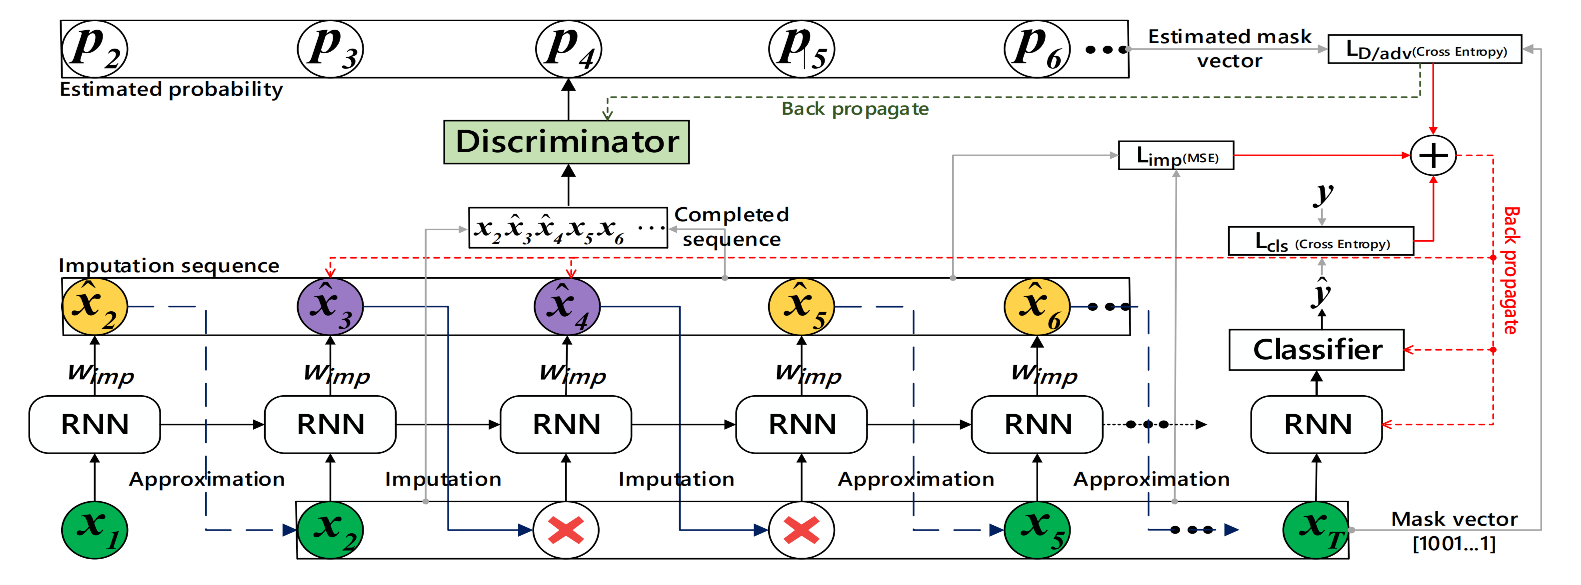
\includegraphics[width=1\textwidth]{ajrnn}
  \caption{The figure shows the proposed AJ-RNN framework. The green units represent revealed inputs, yellow for the output of approximated values, purple for the imputed values, and a red "X" for missing inputs. The dashed links represent the approximation training, while the solid links represent imputation. The discriminator receives a completed vector composed of revealed and imputed values as input, which provides a one-to-one supervisory signal for imputed values $\hat{x_3}$ and $\hat{x_4}$.}
  \label{fig:AJRNNrchitecture}
\end{figure}
\pagebreak
\section{L-TAE}
The paper ``Lightweight Temporal Self-Attention for Classifying Satellite Image Time Series" \cite{LTAE} was written by Vivien Sainte Fare Garnot and Loic Landrieu and published in 2020.

The authors present a new deep learning model for classifying satellite image time series using a modified version of the Temporal Attention Encoder.

In their proposed network, the channels of temporal inputs are distributed among several attention heads operating in parallel. These heads extract specialized temporal features, which are then concatenated into a single representation. The authors show that their approach achieves superior performance compared to other state-of-the-art time-series classification algorithms on an open-access satellite image dataset, while using significantly fewer parameters and reducing computational complexity.

Overall, the paper presents a novel method for classifying satellite image time series that utilizes a lightweight variant of temporal self-attention and outperforms other state-of-the-art approaches.

\subsection{Multi-Headed Self-Attention}

The original version of self-attention, originally developed for text translation as described in \cite{vaswani}, involves three main steps.
First, for each position $t$ in the input sequence, a key-query-value triplet is computed, denoted as $k^{(t)}$, $q^{(t)}$, and $v^{(t)}$, respectively, by applying a shared linear layer to the input $e^{(t)}$.
Second, attention masks are computed representing the compatibility (dot product) between the queries and the keys of previous elements in the sequence. 
Finally, an output is assigned to each position in the sequence, which is the sum of the previous values weighted by the corresponding attention mask.

To allow each head to specialize in detecting specific features of the feature vectors, the self-attention process is performed in parallel for $H$ sets of independent parameters or heads, and the outputs are concatenated.
This approach is used by Rußwurm et al. \cite{russwurm2019self} to embed sequences of satellite observations by max-pooling the resulting sequence of outputs in the temporal dimension.

Garnot et al. \cite{garnot2020satellite} introduce a modified self-attention scheme called the Temporal Attention Encoder (TAE).
First, they propose to use the input embeddings directly as values (i.e., $v^{(t)} = e^{(t)}$), which takes advantage of the end-to-end training of the image embedding functions along with the TAE.
They also define a single master query $\hat{q}$ for each sequence, which is computed from the temporal average of the queries.
The master query is compared to the key sequence to generate a single attention mask of dimension $T$, which is used to weight the temporal average of the values into a single feature vector.

\subsection{Model}
Their work is an extension of previous efforts to adapt multi-head self-attention for sequence embedding.
The primary goal is to optimize efficiency, especially with respect to the number of parameters and the computational load.

\begin{figure}[H]
  \centering
  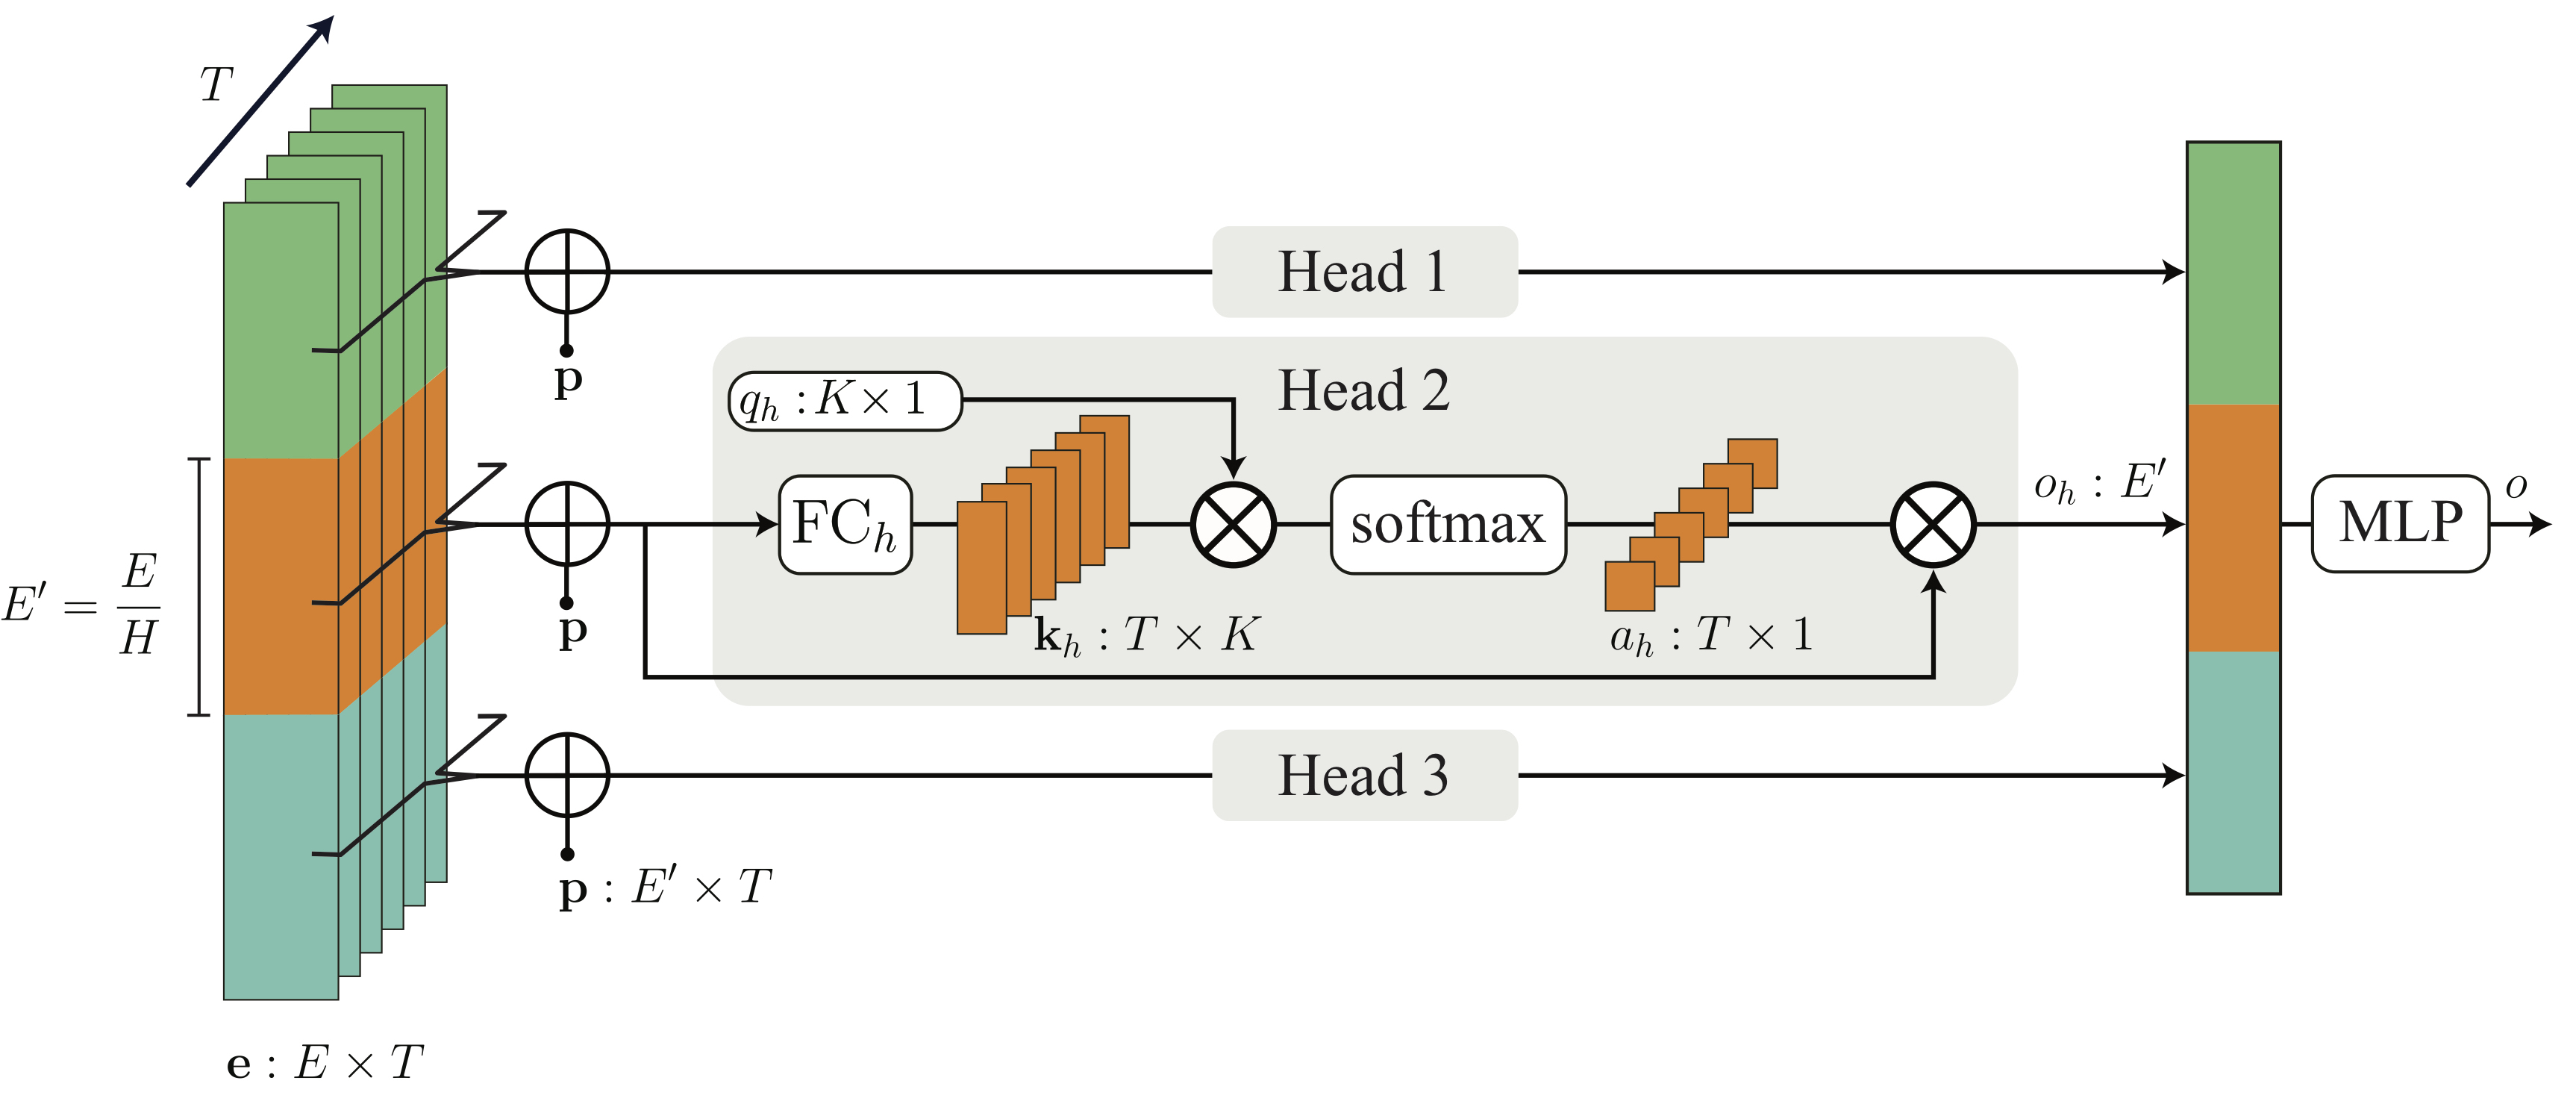
\includegraphics[width=1\textwidth]{LTAE}
  \caption{Light Temporal Attention Encoder  (L-TAE) module processing an input sequence e of $T$ vectors of
  size $E$, with $H = 3$ heads and keys of size $K$. The channels of the input embeddings
  are distributed among heads. Each head uses a learnt query $\hat{q_h}$, while a linear layer
  $FC_h$ maps inputs to keys. The outputs of all heads are concatenated into a vector with
  the same size as the input embeddings, regardless of the number of heads \cite{LTAE}}
  \label{fig:LTAErchitecture}
\end{figure}

\begin{paragraph}{Channel Grouping} 
The proposal is to divide the $E$ channels of the input elements into $H$ groups of size $E' = E/H$ following the approach of Wu et al. \cite{wu2018group}, where $H$ refers to the number of heads. The groups of input channels for the $h$-th group of the t-th element of the input sequence (\ref{eq:LTAE1}) are denoted by $e^{(t)}_h$.

To encode the number of days elapsed since the beginning of the sequence, an $E'$-dimensional positional vector $p$ with a characteristic scale $\tau = 1000$ is used (\ref{eq:LTAE2}).
To enable each head to access this information, the vector $p$ is replicated and added to every channel group.
This approach allows each head to work in parallel on its corresponding group of channels, reducing the computational expense of calculating keys and queries. Additionally, it allows each head to specialize alongside its channel group and avoid redundant operations between heads.
\end{paragraph} 

\begin{paragraph}{Query-as-Parameter} 
The K-dimensional master query $q_h$ of each head $h$ is defined as a model parameter instead of the results of a linear layer.
This approach has the immediate advantage of reducing the number of parameters required.
Although this method lacks flexibility, it is compensated by the greater number of heads available.
\end{paragraph} 

\begin{paragraph}{Attention Masks}
The approach involves using a learned linear layer (\ref{eq:LTAE3}) solely for obtaining the keys, bypassing the values $(v^{(t)} = e^{(t)})$, and employing model parameters for the queries.
For each head $h$, the attention masks $a_h \in [0, 1]^T$ are obtained by scaling the softmax of the dot product between the keys and the master query (\ref{eq:LTAE4}).
The outputs $o_h$ of each head are determined by summing the corresponding inputs weighted by the attention mask $a_h$ along the temporal dimension (\ref{eq:LTAE5}).
Following this step, the outputs of each head are concatenated to form a vector of size $E$, which is then processed through a multi-layer perceptron MLP to achieve the desired size (\ref{eq:LTAE6}).

A schematic representation of the network is provided in Figure \ref{fig:LTAErchitecture}.
In summary, the various steps of the L-TAE method can be summarized by the following operations for $h = 1...H$ and $t = 1...T$:

\begin{align}
  e^{(t)}_h &= e^{(t)}[(h-1) E'...hE']                                  \label{eq:LTAE1}\\
  [p^{(t)}] &= sin(day(t)/\tau^{\frac{i}{E'}})                          \label{eq:LTAE2}\\
  k^{(t)}_h &= FC_h(e^{(t)}_h + p^{(t)})                                \label{eq:LTAE3}\\
  a_h       &= softmax \Bigr(\frac{1}{\sqrt{K}} \Bigr[[q_h \cdot k^{(t)}_h\Bigr]^T_{t=1}\Bigr) \label{eq:LTAE4}\\
  o_h       &= \sum_{t=1}^{T} a_h[t] (e^{(t)}_h + p^{(t)})              \label{eq:LTAE5}\\
  o         &= MLP([o_1,...,o_H]).                                      \label{eq:LTAE6}
\end{align}

\end{paragraph}

\begin{paragraph}{Spatio-temporal classifier}
The L-TAE temporal encoder is designed to be trained together with a spatial encoding module and a decoder module in an end-to-end manner (\ref{eq:LTAE7}).
  
The spatial encoder $S$ is responsible for mapping a sequence of raw inputs $X^{(t)}$ to a sequence of learned features $e^{(t)}$, computed independently at each position of the sequence.
On the other hand, the decoder $D$ is responsible for mapping the output $o$ of the L-TAE to a target vector $y$, which can be class logits in the case of a classification task.
\end{paragraph}

\begin{equation}
  \label{eq:LTAE7}
  \Bigr[X^{(t)}\Bigr]^T_{t=1} \quad \xrightarrow{S} \quad \Bigr[e^{(t)}\Bigr]^T_{t=1} \quad \xrightarrow{L\mbox{--}TAE} \quad o \quad \xrightarrow{D} \quad y
\end{equation}
\pagebreak